\documentclass{ximera}
%\def\sectionautorefname~#1\null{\S#1\null}
%\def\subsectionautorefname~#1\null{\S#1\null}
\title{Setting up the repository}
%\def\itemautorefname~#1\null{#1\null}
\begin{document}
\begin{abstract}
Instructions for setting up a repository containing course materials.
\end{abstract}
\maketitle


\subsection{Setting up a Ximera repository from scratch}
This section describes how to create a course from scratch.
\begin{enumerate}
\item\label{Mkdir} Create a directory for your course files
and change to that directory.
In this example, we will create a directory called
\verb|anExampleCourse|.
Open a terminal session and type the following commands.
\begin{verbatim}
mkdir anExampleCourse
cd anExampleCourse 
mkdir theFirstActivity
mkdir theExampleCourse
cd theExampleCourse 
\end{verbatim}
\item A \link[Ximera]{http://ximera.osu.edu} course consists of a
   \item directory (\verb!anExampleCourse!)  containing a directories
     (\verb!theFirstActivity!, \verb!theExampleCourse!) that all
     contain \LaTeX\ files using the \verb!ximera! document class
     \textbf{except for exactly one} that contains a \LaTeX\ file
     using the \verb!xourse! document class
     (\verb!theExampleCourse.tex!). We describe
     \verb!theExampleCourse.tex! now:

\begin{verbatim}
\documentclass{xourse}

\title{An example course}%% This is the Name of your course, personalize it!

\begin{document}
\begin{abstract} %% This describes your course
This is a Ximera activity explaining how to get started with Ximera for course instructors.
\end{abstract}
\maketitle

%% Here we have a listing of the activities. 
\activity{../theFirstActivity/theFirstActivity}

\end{document}
\end{verbatim}

Now make sure you are in the directory \verb!theExampleCourse! and
type in the terminal \verb!git add theExampleCourse.tex!. This makes
our new file (and the directory containing it, part of our git
repository.


\begin{remark}
In general the file with the \verb!xourse! document class specifies
course information such as the name of the course, a description of
the course, and the names of all \LaTeX\ activity files comprising the
course, in the order they should be presented to students.  In
addition to a name and a description, \verb!theExampleCourse.tex!
  above specifies that there is one activity file
  \verb!theFirstActivity.tex!, written with or without the extension
  \verb!.tex!, and located in a directory called
  \verb!theFirstActivity!.  We will create this file and directory in
  the following step.

Generally courses should contain more than one activity. We recommend
placing each activity in a directory of the same name.  This
facilitates sharing activities among collaborators and makes reusing
existing activities easier.
%Later in this course, we will see examples of
%how to borrow existing activities from other courses
%rather than starting from scratch. 
We also recommend that the directory and the \LaTeX\ file have exactly
the same name as the title of the activity,
with all spaces removed and all words other than the first word
capitalized. So for example, if the title of the
activity were \verb!Plants native to Ohio!
the \LaTeX\ file \verb!plantsNativeToOhio.tex!
would be located in a directory called
\verb!plantsNativeToOhio!.
\end{remark}

\item In your terminal create a new directory
in the \verb!anExampleCourse! directory
called \verb!theFirstActivity!. The \verb!theFirstActivity!
directory should contain a file called \verb!theFirstActivity.tex!.
This can be accomplished by
executing the commands below.
\begin{verbatim}
mkdir theFirstActivity 
cd theFirstActivity 
touch theFirstActivity.tex
git add theFirstActivity.tex
\end{verbatim}

\item\label{FirstExercise}
Using your text editor, open \verb!theFirstActivity.tex!
and paste in the following text. Then save the file.
\begin{verbatim}
\documentclass{ximera}
\title{The First Activity}
\begin{document}
\begin{abstract}
This activity deals with \verb!Ximera! activities.
\end{abstract}
\maketitle
\end{document}
\end{verbatim}

\begin{remark}
An activity should be composed as a regular
\LaTeX\ file in the document class \verb!ximera!.
It should contain the title of the activity and an abstract.
These will both appear on the course website in the navigation area,
so the abstract should be short.
At this stage your activity contains
a title and an abstract, but is otherwise blank.
\end{remark}

\item\label{GithubCreate} Log into your
  \link[github.com]{http://github.com} account and create a repository
  with the name \verb!anExampleCourse!  by clicking the \verb!+! by
  your account name, as shown in the image below.

\begin{image}
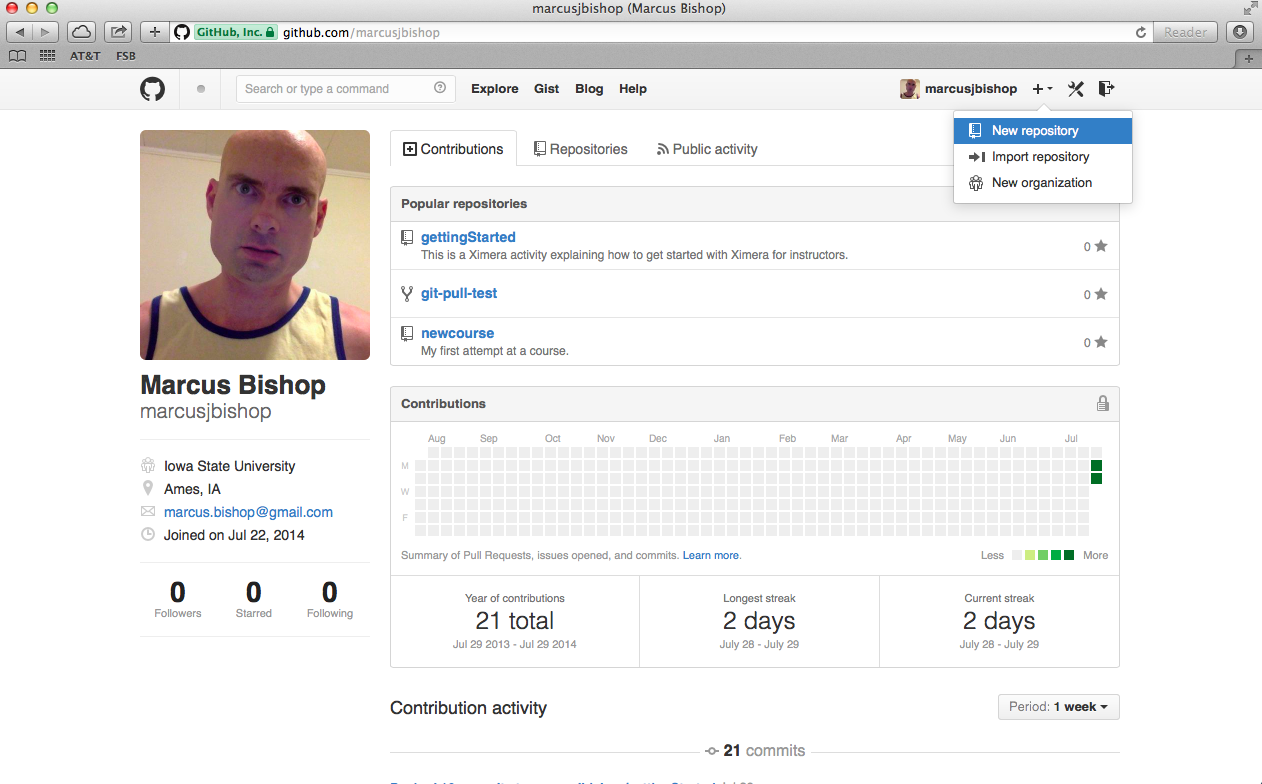
\includegraphics[scale=.3]{RepoInit.png}
\end{image}

After selecting \verb!New repository! from the dropdown menu, a new
page appears with a field named \verb!Repository name!. Enter
\verb!anExampleCourse! into this field and
accept all the default settings by pressing the green
\verb!Create Repository! button.
\begin{image}
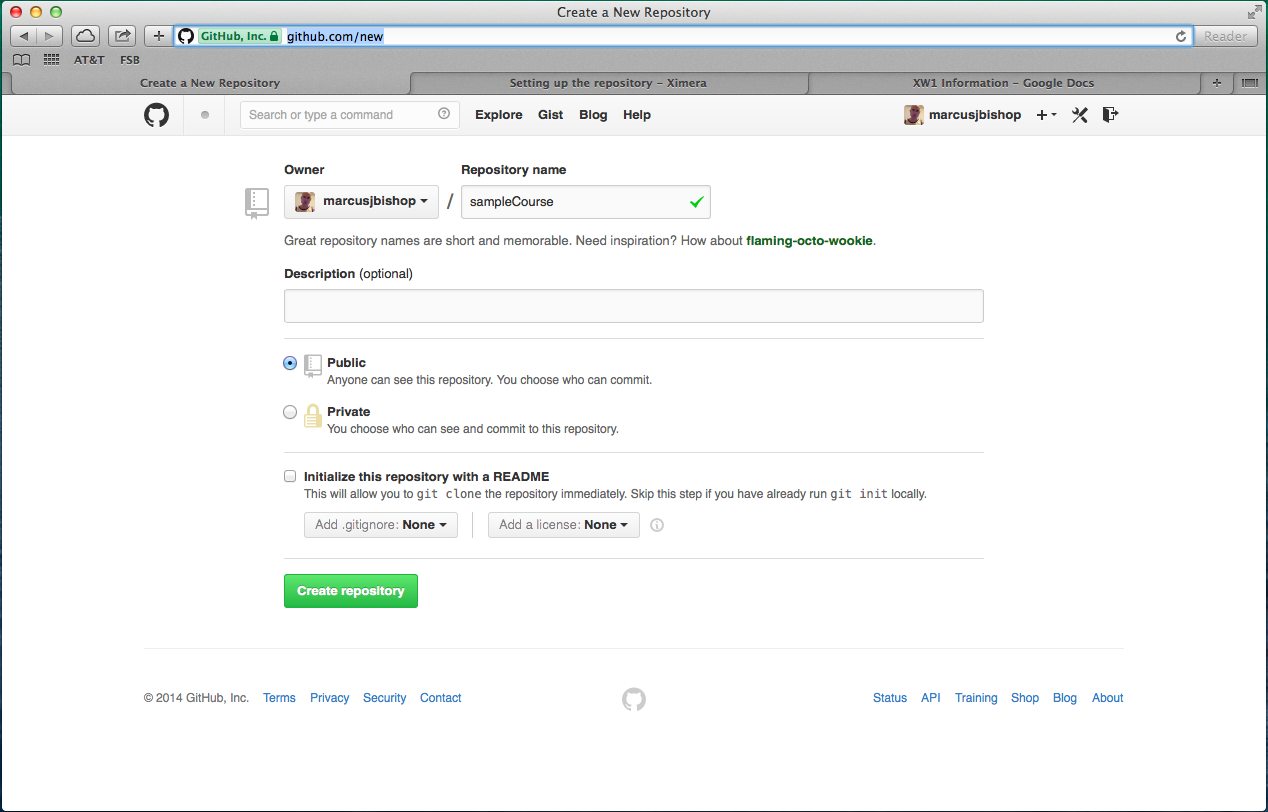
\includegraphics[scale=.3]{CreateRepo.png}
\end{image}
\link[github.com]{http://github.com}
will respond by printing additional commands similar to
those shown below.
\begin{verbatim}
touch README.md
git init
git add README.md
git commit -m "first commit"
git remote add origin https://github.com/marcusjbishop/anExampleCourse.git
git push -u origin master
\end{verbatim}
Before executing these commands, return
to your terminal and ensure that your current directory is
\verb!anExampleCourse!. 
If your current directory is \verb!theFirstActivity!
from the previous step you can change to its parent directory by typing
\begin{verbatim}
cd ..
\end{verbatim}
Now execute the commands returned by
\link[github.com]{http://github.com}.

\begin{remark}
Note that your username appears in the fifth line
of these commands in place of \verb!marcusjbishop!.
Note also the \verb!s! in \verb!https!.
These commands initialize the repository on \link[github.com]{http://github.com}
and create an empty file named \verb!README.md!
in the \verb!anExampleCourse! directory.
\end{remark}

\item This step is optional. Type a
description of your course in the file
\verb!README.md!.

\begin{remark}
The content of \verb!README.md! will appear only on
\link[github.com]{http://github.com}
This file is meant to provide a description of your project
to other developers.
\end{remark}

\item In order to have your course served by
  \link[ximera.osu.edu/]{http://ximera.osu.edu/} you need permission
  to publish.  Request permission by e-mailing
  \link[ximera@math.osu.edu]{mailto:ximera@math.osu.edu}.

\item Go to your profile on
  \link[ximera.osu.edu/]{http://ximera.osu.edu/}, create a key and
  secret, and in a terminal, run
\begin{verbatim}
xake login
\end{verbatim}
and paste in your key and secret.

\item This is a good point to add some further content in the
  form of a simple exercise.  Update the file
  \verb!theFirstActivity.tex!  you created above so that it looks like
  the following.

\begin{verbatim}
\documentclass{ximera}
\title{The First Activity}
\begin{document}
\begin{abstract}
This activity deals with \verb!Ximera! activities.
\end{abstract}
\maketitle
This activity is about creative work.
\begin{exercise}
  Choose the best place to work on mathematics.
  \begin{multipleChoice}
    \choice{At the library}
    \choice[correct]{At the caf\'e}
    \choice{In your office}
  \end{multipleChoice}
\end{exercise}
\end{document}
\end{verbatim}
\begin{remark}
The edits above insert
a multiple-choice question into the \verb!theFirstActivity!
activity. See the {\sf Question and answer types}
activity later in this tutorial
for more information on creating exercises.
\end{remark}

\item Change to the directory \verb!anExampleCourse!
and execute the following commands.
\begin{verbatim}
git commit -m "Added an exercise"
xake bake
xake publish
\end{verbatim}
If everything went well, you should see a URL printed on the terminal.
If not, see the {\sf Troubleshooting} activity in this tutorial or
send your questions to
\link[ximera@math.osu.edu]{mailto:ximera@math.osu.edu}.
\begin{remark} The commands above inform 
\link[git]{http://git-scm.com} that changes have been made to your
repository and communicates them to
\link[github.com]{http://github.com} which in turn communicates them
to \link[ximera.osu.ed]{http://ximera.osu.edu}.  You should execute
similar commands whenever you change files in your repository.
\end{remark}
\end{enumerate}

\subsection{Creating further activities}
From here you can create further \link[Ximera]{http://ximera.osu.edu}
activities as in step~\autoref{FirstExercise}.  You should issue a
\verb!git add! command after creating a new file or directory and a
\verb!git commit!  command followed by a \verb!git push! command
periodically to transmit your most recent changes to
\link[github.com]{http://github.com}.  You should also add the name of
your activity file to the \verb!xourse! file in the position relative
to other activities where you want the activity to appear.  Observe
however that once the filename appears in the \verb!xourse!  file the
corresponding activity will appear to students. It might therefore be
preferable to create a separate branch on GitHub until the activity is
ready for students.  During the editing phase you still view the
activity by processing it with \LaTeX\ and inspecting the resulting
PDF file, which might be helpful in any case for finding and
correcting mistakes.

\subsection{Other ways to set up a Ximera repository}\label{ForkClone}
There are other ways to create a \link[Ximera]{http://ximera.osu.edu}
course.  One possibility is to begin by creating the repository on
\link[github.com]{http://github.com} as in step~\autoref{GithubCreate}
above.  Then instead of executing the commands that follow to
initialize the local copy of the repository, you could {\em clone} the
copy on \link[github.com]{http://github.com} using a \verb!git clone!
  command.  Alternately you could {\em fork} an existing repository,
  either your own or someone else's.  See the \link[git
    manual]{http://git-scm.com} for more information about the
  \verb!clone! and \verb!fork! commands.  Both possibilities above
  obviate step \autoref{Mkdir} since cloning or forking a
  \link[git]{http://git-scm.com} repository creates a local directory
  and initializes it as a \link[git]{http://git-scm.com} repository.

Still another possibility is to create and edit {\em all} files and
directories directly on the \link[github.com]{http://github.com} web
site.  In this way you could produce an entire
\link[Ximera]{http://ximera.osu.edu} course {\em without} a local copy
of the repository.  This would have the advantage of not requiring the
instructor to install the \link[git]{http://git-scm.com} or
\link[\LaTeX]{http://texlive.org} software or to learn any of the
\link[git]{http://git-scm.com} or Unix commands above. This could be
useful when working temporarily on someone else's computer, for
example.

\end{document}
